
\newpage
\chapter{ساز و کار های درون یک لایه نورونی}
\section{مقدمه}
    \subsection{مجموعه داده مورد استفاده}
        در این پروژه، برای الگو های ساده، از الگوی 
        \ref{fig:simple-pattern1} 
        و 
        \ref{fig:simple-pattern2}
        استفاده می‌کنیم و برای الگو های پیچیده تر از از مخزن دانشگاه واترلو
        \footnote{\href{https://links.uwaterloo.ca/Repository.html}{مخزن تصاویر دانشگاه واترلو}}
        با نسبت اندازه های مختلف استفاده می‌کنیم. این تصاویر همگی سیاه و سفید هستند. از این رو میتوانیم کل تصویر را به صورت یک آرایه درنظر بگیریم، به طوری که سطر های تصویر را پشت سر هم ردیف می‌کنیم. کدگذاری مورد استفاده در این پروژه نیز، کد گذاری پواسون می‌باشد.
        \begin{figure}[!ht]
            \centering
            \begin{adjustbox}{minipage=\linewidth,scale=0.4}
                \begin{subfigure}[b]{0.4\textwidth}
                    \centering
                    
\includegraphics[width=\textwidth]{images/pattern1.png}
                    \caption{الگوی ورودی ساده شماره ۱}
                    \label{fig:simple-pattern1}
                \end{subfigure}
                \hfill
                \begin{subfigure}[b]{0.4\textwidth}
                    \centering
                    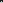
\includegraphics[width=\textwidth]{images/pattern2.png}
                    \caption{الگوی ورودی ساده شماره ۲}
                    \label{fig:simple-pattern2}
                \end{subfigure}
                \vfill
                \begin{subfigure}[b]{0.4\textwidth}
                    \centering
                    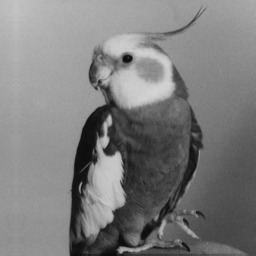
\includegraphics[width=\textwidth]{images/bird.jpg}
                    \caption{یک نمونه تصویر از مخزن دانشگاه واترلو}
                    \label{fig:waterloo-sample-original}
                \end{subfigure}
                \hfill
                \begin{subfigure}[b]{0.4\textwidth}
                    \centering
                    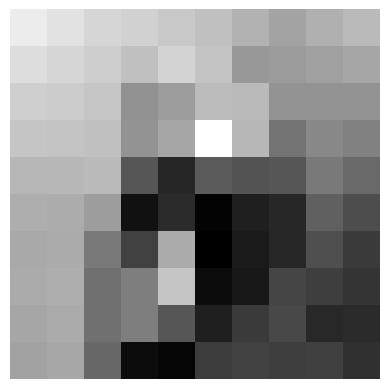
\includegraphics[width=\textwidth]{images/bird-resized.jpg}
                    \caption{تصویر 
                    \ref{fig:waterloo-sample-original}
                    از مخزن دانشگاه واترلو که کوچکتر شده است.}
                    \label{fig:waterloo-sample-resized}
                \end{subfigure}
            \end{adjustbox}
            \caption{مجموعه داده مورد استفاده}
            \label{fig:dataset}
        \end{figure}
    \subsection{یک مدل ساده}
        در این پروژه می‌خواهیم با ساز و کار های موجود بین نورون های یک لایه آشنا شویم و تاثیر آن ها را بر فرآیند یادگیری بررسی کنیم. برای اینکار لازم است ابتدا، یک آزمایش ساده برای حالتی که هیچ یک از این ساز و کار ها درون لایه ها وجود ندارد انجام دهیم تا نتایج را بهتر با‌آن مقایسه کنیم. همانطور که در فایل پروژه نیز آمده است، در شبکه مورد نظر، تنها یک لایه ورودی و یک لایه خروجی در نظر میگیریم. سپس یک سیناپس با اتصال کامل و وزن های اولیه تصادفی بین این دو لایه ایجاد می‌کنیم. همچنین از قانون یادگیری انعطاف‌پذیری وابسته به زمان ضربه 
        ($STDP$\footnote{\lr{Spike-Timing-Dependent Plasticity}})
        برای آموزش شبکه استفاده می‌کنیم. از آنجا که این آزمایش به عنوان یک مرجع برای مقایسه در نظر گرفته می‌شود، رفتار دندریت ها را نیز یک رفتار ساده در نظر میگیریم. در نهایت، شبیه سازی را برای ۱۰۰۰ تکرار انجام می‌دهیم.
        همانطور که پروژه قبل نیز ملاحظه کردیم، قانون یادگیری 
        $STDP$ 
        به تنهایی نمی‌تواند در یادگیری الگو ها به خوبی 
        $RSTDP$ 
        عمل کند. هر چند که این قانون، مطابق شکل 
        \ref{fig:part1-simple-stdp-correct} 
        توانسته است الگو های ورودی را به خوبی یاد بگیرد، اما این یادگیری پایدار نیست و به ازای تکرار ها مختلف ممکن است به طرق متفاوت عمل کند.
        (شکل \ref{fig:part1-simple-stdp-multiple-runtime})
        \begin{figure}[!ht]
            \centering
            \includegraphics[width=0.9\textwidth]{plots/part1-simple-stdp-correct.pdf} 
            \captionsetup{width=.9\linewidth}
            \caption{\textbf{یک شبکه ساده با قانون یادگیری 
            $STDP$ ساده و بدون ساز و کار اضافه.} برای درک بهتر و تحلیل ساز و کار های درون یک لایه، بهتر است یک شبکه ساده در نظر گرفته و رفتار آن را با شبکه هایی که ساز و کار به آن ها اضافه می‌شود مقایسه کنم. همانطور که در پروژه قبل دیدیم، قانون یادگیری 
            $STDP$ 
            می‌تواند در یادگیری الگو های ساده، تا حد قابل قبولی عمل کند. هر چند این عملکرد ممکن است پایدار نباشد.(شکل \ref{fig:part1-simple-stdp-multiple-runtime})}
            \label{fig:part1-simple-stdp-correct}
        \end{figure}

        \begin{figure}[!ht]
            \centering
            \includegraphics[width=0.9\textwidth]{plots/part1-simple-stdp-multiple-runtime-2.pdf} 
            \captionsetup{width=.9\linewidth}
            \caption{\textbf{مقایسه نتایج شبیه سازی های مختلف شبکه تنها با قانون یادگیری $STDP$.} همانطور که در شکل بالا نیز مشاهده می‌کنیم، اجرای شبیه سازی یک شبکه یکسان که تنها قانون یادگیری 
            $STDP$ 
            را دارد، می‌تواند منجر به نتایج متفاوت شود. در شکل بالا، در شبیه سازی اول، شبکه نتوانسته است به خوبی الگو ها را یاد بگیرد، اما شبیه سازی های دوم و سوم عملکرد خوبی داشته‌اند.}
            \label{fig:part1-simple-stdp-multiple-runtime}
        \end{figure}

\clearpage
\section{افزودن ساز و کار مهار جانبی (\lr{Lateral Inhibition})}
    در علوم اعصاب، مهار یا بازداری جانبی ظرفیت یک نورون برانگیخته برای کاهش فعالیت همسایگان خود است. مهار جانبی گسترش پتانسیل های عمل را از نورون های برانگیخته به نورون های همسایه در جهت جانبی غیرفعال می کند. این عمل یک کنتراست در تحریک ایجاد می کند که باعث افزایش ادراک حسی می شود و به آن تضاد جانبی نیز گفته می شود و عمدتاً در فرآیندهای بینایی، بلکه در پردازش لمسی، شنوایی و حتی بویایی نیز رخ می دهد.
    \cite{Lateral-inhibition-wikipedia}
    \begin{figure}[!ht]
        \centering
        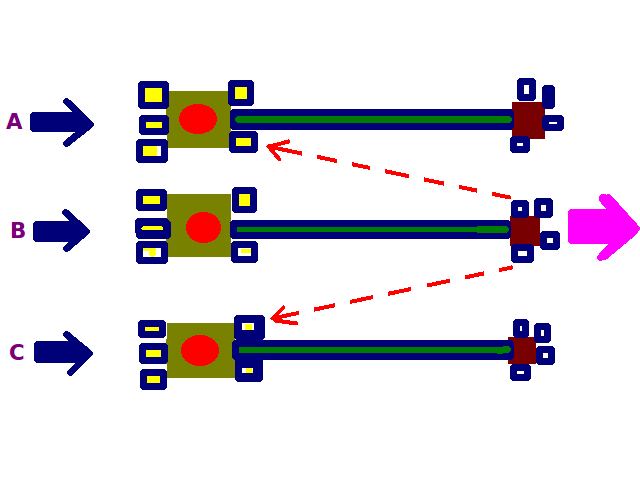
\includegraphics[width=0.6\textwidth]{images/Lateral_Inhibition.png} 
        \captionsetup{width=.8\linewidth}
        \caption{محرکی که بر هر سه نورون تأثیر می‌گذارد، اما بر 
        B
        قوی‌ترین یا اول تأثیر می‌گذارد، اگر B سیگنال‌های جانبی را به همسایگان 
        A و C 
        ارسال کند تا ضربه نزنند، در نتیجه آنها را مهار می‌کند. مهار جانبی در بینایی برای $sharp$ کردن سیگنال‌های مغز 
        (فلش صورتی) 
        استفاده می‌شود.}
        \label{fig:lateral-inhibition}
    \end{figure}

    برای شبیه سازی ساز و کار مهار جانبی، ممکن است بتوان به چندین روش عمل کرد. از آنجا که می‌خواهیم یک نورون برانگیخته همسایگان خود را مهار کند، می‌توان اینکار را از طریق ایجاد یک جریان منفی از سمت این نورون به نورون های همسایه یا پایین آوردن اختلاف پتانسیل آن ها این کار را انجام داد. روشی که درون این پروژه استفاده شده است، همان روشی است که در کتابخانه 
    $CoNeX$ 
    نیز استفاده شده است. شمای کلی این روش، در شکل 
    \ref{fig:lateral-inhibition-scheme}
    که از 
    \cite{Unsupervised-Learning-Lateral-Inhibition} 
    برداشته شده، آمده است.
    \begin{figure}[!ht]
        \centering
        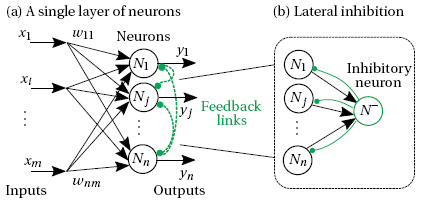
\includegraphics[width=0.6\textwidth]{images/lateral_inhibition_scheme.png} 
        \captionsetup{width=.8\linewidth}
        \caption{\textbf{یک شبکه SNN
        تک لایه با پیوندهای بازخورد }
        (الف)
        نورون های تحریکی 
        $N1، . . . ، Nn$ 
        با پیوندهای بازخوردی در ارتباط هستند که فعالیت های واگرا را در نورون ها تقویت می کند. 
        (ب) 
        پیوندهای بازخورد اغلب ساز و کار مهار جانبی را اجرا می کنند، که در آن یک نورون بازدارنده اضافی 
        N- 
        نورون های تحریکی را مهار می کند. 
        (رجوع کنید به \cite{Unsupervised-Learning-Lateral-Inhibition})}
        \label{fig:lateral-inhibition-scheme}
    \end{figure}

    حال که با نحوه ساز و کار مهار جانبی آشنا شدیم، آن را به مدلمان افزوده و آزمایش می‌کنیم. برای اینکار لازم است که یک سیناپس جدید، از لایه خروجی به خودش تشکیل و دهیم، و به آن رفتار مهار جانبی را اضافه کنیم. 
    
    همانطور که در شکل 
    \ref{fig:part1-simple-stdp-lateral-inhibition} 
    نیز ملاحظه می‌کنیم افزودن ساز و کار مهار جانبی به لایه خروجی باعث می‌شود فرایند یادگیری مدل بهبود یابد و نه تنها در مراحل زودتری، بتواند الگو ها را تشخیص دهد، بلکه با تکرار شبیه سازی، با احتمال بیشتری دقت پایداری را حفظ کند. همچنین همانطور که ملاحظه می‌کنیم نمودار شباهت کسینوسی آن به سمت صفر میل می‌کند.

    \begin{figure}[!ht]
        \centering
        \includegraphics[width=0.95\textwidth]{plots/part1-simple-stdp-lateral-inhibition.pdf} 
        \captionsetup{width=.85\linewidth}
        \caption{\textbf{افزودن ساز و کار مهار جانبی به لایه خروجی. } 
        همانطور که در شکل بالا مشاهده می‌کنیم، افزودن ساز و کار مهار جانبی به لایه خروجی، باعث بهبود فرایند یادگیری مدل می‌شود. به طوری که مدل هم در مراحل زودتری الگو ها را تشخیص می‌دهد، و هم با تکرار آزمایش، با احتمال بیشتری نسبت به حالتی که این ساز و کار وجود ندارد پایداری خود را حفظ می‌کند. نکته مهم دیگری که در این شکل مشاهده می‌شود، نمودار شباهت کسینوسی بین وزن های لایه خروجی است. این نمودار در حالتی که این ساز و کار وجود نداشت، پس از اینکه تا حدی کم می‌شد، نزدیک صفر نوسان میکرد، اما با افزودن ساز و کار مهار جانبی، شباهت کسینوسی بعد از حدود ۲۵۰ تکرار به مقدار صفر میل می‌کند.
        }
        \label{fig:part1-simple-stdp-lateral-inhibition}
    \end{figure}

    تکرار آزمایش با الگوی پیچیده تر نیز 
    (مجموعه داده دانشگاه واترلو) 
    نتایج مشابهی به همراه خواهد داشت و مدل توانایی تشخیص الگو ها را همچنان دارد.(شکل \ref{fig:part1-simple-stdp-lateral-inhibition-large-data})

    \begin{figure}[!ht]
        \centering
        \includegraphics[width=0.95\textwidth]{plots/part1-simple-stdp-lateral-inhibition-large-data.pdf} 
        \captionsetup{width=.85\linewidth}
        \caption{\textbf{افزودن ساز و کار مهار جانبی به لایه خروجی: الگو های های پیچیده تر. } 
        مشاهده می‌کنیم حتی با شبیه سازی آزمایش با الگو های پیچیده تر، یعنی تصاویر مجموعه داده دانشگاه واترلو نیز، مدل توانایی خود در تشخیص دادن را از دست نداده است.
        }
        \label{fig:part1-simple-stdp-lateral-inhibition-large-data}
    \end{figure}

    \subsubsection*{نتیجه گیری}
        افزودن ساز و کار مهار جانبی به لایه خروجی، باعث می‌شود توانایی مدل در تشخیص الگو ها بیشتر شود و نورون ها به الگو های متفاوت حساس تر شوند. در ساز و کار مهار جانبی، برانگیخته شدن یک نورون، باعث می‌شود همسایه های خود را مهار کند. از این رو، افزودن این ساز و کار به لایه خروجی، باعث می‌شود هنگامی که یک نورون به یک الگو حساس می‌شود، نورون دیگر را مهار کرده و در نتیجه، تشخیص الگو ها مقداری بهتر شود. هرچند این ساز و کار به تنهایی برای یادگیری انواع مدل ها کافی نیست.

    \subsection{آزمایش مدل با اشتراک متفاوت الگو ها}
        در این قسمت، آزمایش را با میزان اشتراک متفاوت الگو ها تکرار می‌کنیم. برای اینکار، سه مقدار متفاوت 
        $20\%$, $50\%$ و $100\%$
        را بین دو الگو در نظر گرفته و برای هر کدام شبیه سازی را انجام می‌دهیم. مطابق شکل 
        \ref{fig:part1-simple-stdp-lateral-inhibition-different-overlap}
        مشاهده می‌کنیم که با افزودن میزان اشتراک بین الگو های ورودی نیز همچنان مدل توانایی تشخیص دادن الگو ها را دارد. هر چند در مدلی که میزان اشتراک به حداکثر خود رسیده است، مشاهده می‌کنیم که مدل دیرتر الگو ها را تشخیص می‌دهد و همچنین نمودار شباهت کسینوسی آن نیز دیر به سمت صفر میل می‌کند.
        \begin{figure}[!ht]
            \centering
            \includegraphics[width=0.95\textwidth]{plots/part1-simple-stdp-lateral-inhibition-different-overlap.pdf} 
            \captionsetup{width=.85\linewidth}
            \caption{\textbf{ ساز و کار مهار جانبی در لایه خروجی: آزمایش میزان اشتراک متفاوت الگوها} 
            مشاهده می‌کنیم حتی با شبیه سازی آزمایش با میزان اشتراک متفاوت الگو هانیز مدل توانایی خود در تشخیص دادن را از دست نداده است. هرچند در شکل سمت راست که مدل حداکثر اشتراک را در الگو ها دارد، تشخیص دادن در مراحل دیرتری اتفاق می‌افتد، اما در نهایت موفق به تشخیص الگو ها می‌شود. علاوه بر آن، نمودار شباهت کسینوسی نیز دیر به سمت صفر میل می‌کند. در این مدل، بقیه پارامتر ها همانند شکل 
            \ref{fig:part1-simple-stdp-lateral-inhibition-large-data} 
            می‌باشد.
            }
            \label{fig:part1-simple-stdp-lateral-inhibition-different-overlap}
        \end{figure}
    \subsection{نتایج}
        در این قسمت، مدل را با اندازه الگو های مختلف شبیه سازی می‌کنیم و بررسی می‌کنیم که مدل برای چه تعداد ورودی می‌تواند آن ها را تشخیص دهد. مطابق شکل 
        \ref{fig:part1-evaluation-simple-stdp-LI}
        مشاهده می‌کنیم که مدل توانسته است تا حدود 6 الگوی ورودی را به خوبی فرا بگیرد. هر چند ممکن است گاهی با اجرای دوباره نتیجه مطلوب گرفته نشود. اما با بیشتر شدن این تعداد تا ۸ عدد، در اکثر مواقع مدل موفق به یادگیری برخی از این الگو ها نمی‌شود و فقط تعدادی را یاد می‌گیرد.

        
        \begin{figure}[!ht]
            \centering
            \begin{adjustbox}{minipage=\linewidth,scale=1}
                \begin{subfigure}[b]{0.45\textwidth}
                    \centering
                    \includegraphics[width=\textwidth]{plots/with-normalization/part1-evaluation-simple-stdp-LI-2-patterns.pdf}
                    \caption{۲ الگو}
                    \label{fig:part1-evaluation-simple-stdp-LI-2-patterns}
                \end{subfigure}
                \hfill
                \begin{subfigure}[b]{0.45\textwidth}
                    \centering
                    \includegraphics[width=\textwidth]{plots/with-normalization/part1-evaluation-simple-stdp-LI-4-patterns.pdf}
                    \caption{۴ الگو}
                    \label{fig:part1-evaluation-simple-stdp-LI-4-patterns}
                \end{subfigure}
                \vfill
                \begin{subfigure}[b]{0.45\textwidth}
                    \centering
                    \includegraphics[width=\textwidth]{plots/with-normalization/part1-evaluation-simple-stdp-LI-6-patterns.pdf}
                    \caption{۶ الگو}
                    \label{fig:part1-evaluation-simple-stdp-LI-6-patterns}
                \end{subfigure}
                \hfill
                \begin{subfigure}[b]{0.45\textwidth}
                    \centering
                    \includegraphics[width=\textwidth]{plots/with-normalization/part1-evaluation-simple-stdp-LI-8-patterns.pdf}
                    \caption{۸ الگو}
                    \label{fig:part1-evaluation-simple-stdp-LI-8-patterns}
                \end{subfigure}
            \end{adjustbox}
            \caption{\textbf{آزمایش مدل با تعداد الگو های متفاوت.}در این آزمایش یک مدل ترین شده روی الگو ها را، به اندازه یک بار ورودی دادن همه الگو ها شبیه سازی می‌کنیم. 
            (تعداد باری که هر الگو را مدل دیده است در هر آزمایش برابر است.) 
            مطابق شکل مشاهده می‌کنیم که مدل توانسته است تا حدود ۶ الگو را به خوبی تشخیص دهد. هر چند این تشخیص ممکن است گاهی در تکرار شبیه سازی موفق نشود. اما هنگامی که مدل را با ۸ الگو آزمایش می‌کنیم مشاهده می‌کنیم که بعضی از الگو ها تشخیص داده نشده اند و نورون های خروجی به کلی ضربه نزده اند. در ادامه خواهیم دید برای جلوگیری از این مشکل
            (که بعضی نورون ها در زمان ورودی گرفتن کل الگو ها ضربه‌ای نزنند.) 
            چه ساز و کار هایی به کمک ما خواهند آمد.}
            \label{fig:part1-evaluation-simple-stdp-LI}
        \end{figure}
        \footnotetext{برای تشخیص عملکرد مدل، دقت کنید در هر بازه‌ای که یک نورون برای الگویی ضربه زده است، نورون های دیگر ضربه‌ای نزده‌اند همچنین هر نورون، در زمان ورودی دادن فقط برای یک الگو ضربه زده است.}

\clearpage
\section{k~-برنده همه چیز را می‌گیرند(K-Winners-Take-All)}
    ساز و کار 
    K-winners-take-all (KWTA) 
    در شبکه‌های عصبی ضربه‌ای
    (یا حتی مصنوعی)
    شکلی از یادگیری رقابتی است که به تعیین اینکه کدام نورون‌ها در یک شبکه به شدت در پاسخ به ورودی‌های خاص فعال می‌شوند کمک می‌کند.
    در زمینه شبکه‌های عصبی ضربه‌ای، که در آن سعی می‌کنیم از نحوه عملکرد نورون‌های واقعی الهام بگیریم، ساز و کار 
    KWTA 
    با اجازه دادن به نورون‌ها برای رقابت بر اساس پتانسیل‌های غشایی یا سرعت ضربه زدن عمل می‌کند. می‌دانیم هر نورون در یک شبکه جریان را دریافت می کند و این جریان ورودی بر پتانسیل آنها تأثیر می گذارد. نورون هایی که به آستانه خاصی می رسند ضربه می‌زنند. از این رو در پیاده سازی 
    KWTA، 
    از بین تمام نورون‌های یک لایه یا گروه خاص، فقط 
    $k$ 
    نورونی که پتانسیل‌شان بالاتر است 
    (یا آن‌هایی که به شدت افزایش یافته اند) 
    مجاز به فعال ماندن یا "برنده شدن" هستند. بقیه سرکوب می شوند یا فعالیت آنها کاهش می یابد، از این رو اصطلاح "برنده ها همه چیز را می گیرند" برای آن به کار برده می‌شود.
    ساز و کار 
    KWTA 
    معمولاً از طریق روش‌های مختلفی مانند بازخورد مهاری، که در آن نورون‌ها فعالیت نورون‌های دیگر را در مجاورت خود مهار می‌کنند، یا از طریق طراحی شبکه که خود معماری تضمین می‌کند که فقط 
    $k$ 
    نورون‌ برتر می‌توانند در هر نقطه فعال باقی بمانند، انجام می‌شود. زمان. این رویکرد را می توان به عنوان شکلی از رقابت بین نورون ها دید که یک ویژگی اساسی سیستم های عصبی بیولوژیکی است و برای کارهایی مانند تشخیص الگو و فرآیندهای تصمیم گیری در هر دو سیستم طبیعی و مصنوعی بسیار مهم است. خلاصه این مفهوم در شکل 
    \ref{fig:k-winners-take-all-schematic}
    آمده است.

    \begin{figure}[!ht]
        \centering
        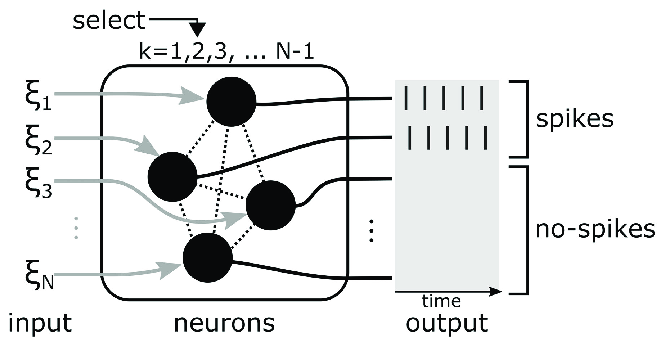
\includegraphics[width=0.6\textwidth]{images/k-winners-take-all-schematic.png} 
        \captionsetup{width=.7\linewidth}
        \caption{\textbf{ ساز و کار 
        «~k~-برنده همه چیز را می‌گیرند».} در هر مرحله از شبیه سازی، فقط آن نورون‌هایی که بزرگترین ورودی را دریافت می‌کنند، ضربه می‌زنند، در حالی که ضربه های همه نورون‌های دیگر به صورت پویا سرکوب می‌شوند.
        }
        \label{fig:k-winners-take-all-schematic}
    \end{figure}

    حال می‌خواهیم این ساز و کار را به شبکه‌مان اضافه کنیم. ابتدا، حالتی را در نظر می‌گیریم که در آن شبکه، از یک لایه ورودی و خروجی و یک سیناپس از لایه ورودی به لایه خروجی استفاده می‌کند. همچنین مشابه قسمت قبل، از قانون یادگیری 
    $STDP$ 
    برای آموزش مدل استفاده می‌کنیم. همانطور که در شکل 
    \ref{fig:part1-simple-stdp-kwta}
    نیز ملاحظه می‌کنیم، افزودن ساز و کار 
    k-winners-take-all 
    به لایه خروجی باعث می‌شود در همان مراحل اولیه، مدل الگو ها را یاد بگیرد. هر چند در این حالت نیز ممکن است در برخی شبیه سازی ها مدل نتواند الگو ها ها را به خوبی یاد بگیرد، اما قرار گرفتن این ساز و کار  در کنار ساز و کار های دیگر که بررسی کردیم یا بررسی خواهیم کرد، توانایی مدل را افزایش خواهد داد. همانطور که از شکل برمی‌آید، اضافه کردن این ساز و کار باعث شده است تمایز وزن های بین نورون ها را شاهد باشیم و همچنین شباهت کسینوسی نسبت به حالت بدون ساز و کار یا با ساز و کار مهار جانبی، زودتر به صفر میل کند.

    \begin{figure}[!ht]
        \centering
        \includegraphics[width=0.95\textwidth]{plots/part1-simple-stdp-kwta.pdf} 
        \captionsetup{width=.85\linewidth}
        \caption{\textbf{اضافه کردن ساز و کار 
        k-winners-take-all
        به تنهایی در لایه خروجی یک شبکه ساده. } 
        مشاهده می‌کنیم که شبکه توانسته است به خوبی الگو های ورودی را یاد بگیرد. نسبت به حالتی که ساز و کاری وجود نداشت یا حالتی که ساز و کار مهار جانبی داشتیم، یاد گرفتن الگو ها زودتر اتفاق افتاده و همچنین شباهت کسینوسی زودتر به سمت صفر میل کرده است. 
        }
        \label{fig:part1-simple-stdp-kwta}
    \end{figure}

    \paragraph*{مقایسه ولتاژ} در این پاراگراف می‌خواهیم دو ساز و کار مهار جانبی و برنده-همه-چیز-را-می‌گیرد را از نظر تاثیر روی ولتاژ مقایسه کنیم. طبق شکل  
    \ref{fig:part1-simple-stdp-KWTA-and-LI-voltage-compare} 
    مشاهده می‌کنیم که نحوه تاثیر این دو ساز وکار بر روی ولتاژ متفاوت است بدین صورت که ولتاژ نورون های سرکوب شده در ساز و کار مهار جانبی، توسط جریان کاهش می‌یابد
    (یک جریان منفی به نورون ها وارد می‌شود) 
    در حالی که در ساز و کار برنده-همه-چیز-را-می‌گیرد این اتفاق به طور مستقیم و ناگهانی در پیاده سازی رخ می‌دهد. دانستن این نکته ممکن است در ساز و کار دیگری که در ادامه آزمایش می‌کنیم،
    (هم‌ایستایی مبتنی بر ولتاژ) 
    مفید باشد.
    
    \begin{figure}[!ht]
        \centering
        % \begin{adjustbox}{minipage=\linewidth,scale=0.5}
            \begin{subfigure}[b]{0.8\textwidth}
                \centering
                \includegraphics[width=\textwidth]{plots/part1-simple-stdp-sample-input-patterns.pdf}
                \caption{\textbf{الگو های ورودی.}}
                \label{fig:part1-simple-stdp-sample-input-patterns}
            \end{subfigure}
            \vfill
            \begin{subfigure}[b]{0.8\textwidth}
                \centering
                \includegraphics[width=\textwidth]{plots/part1-simple-stdp-kwta-voltage.pdf}
                \caption{\textbf{شبکه ساده به همراه ساز و کار مهار جانبی: نمودار ولتاژ دو نورون لایه خروجی.}}
                \label{fig:part1-simple-stdp-kwta-voltage}
            \end{subfigure}
            \vfill
            \begin{subfigure}[b]{0.8\textwidth}
                \centering
                \includegraphics[width=\textwidth]{plots/part1-simple-stdp-lateral-inhibition-voltage.pdf}
                \caption{\textbf{شبکه ساده به همراه ساز و کار 
                k-winners-take-all:
                نمودار ولتاژ دو نورون لایه خروجی.}}
                \label{fig:part1-simple-stdp-kwta-voltage}
            \end{subfigure}
        % \end{adjustbox}
        \caption{\textbf{مقایسه ولتاژ در شبکه با ساز و کار مهار جانبی یا 
        k-winners-take-all.} در شکل بالا، مقایسه ولتاژ در دو شبکه با قانون 
        STDP 
        که یکی دارای ساز و کار مهار جانبی و دیگری دارای ساز و کار 
        k-winners-take-all 
        هستند آمده است. مطابق شکل ملاحظه می‌کنیم که در شبکه ای که مهار جانبی وجود دارد، به دلیل اینکه سرکوب کردن ضربه زدن نورون های همسایه توسط جریان صورت می‌گیرد، ملاحظه می‌کنیم که ولتاژ در زمان هایی که ورودی های مختلف داده می‌شود، یکی درمیان به علت گرفتن جریان منفی زیاد، تا $-90$ درجه کم می‌شوند در حالی که در ساز و کار 
        k-winners-take-all 
        ولتاژ به طور ناگهانی در پیاده سازی برابر با ولتاژ حالت استراحت مقدار می‌شود.}
        \label{fig:part1-simple-stdp-KWTA-and-LI-voltage-compare}
    \end{figure}


    حال به لایه خروجی، ساز و کار مهار جانبی که در بخش قبل انجام دادیم را نیز اضافه می‌کنیم تا رفتار مدل را در حضور هر دو ساز و کار بررسی کنیم. مطابق شکل 
    \ref{fig:part1-simple-stdp-kwta-lateral-inhibtion}
    مشاهده می‌کنیم که با داشتن هر دو ساز و کار 
    k-winners-take-all 
    و مهار جانبی، مدل به خوبی توانسته است دو الگو را تشخیص دهد. مطابق شکل، دریافت می‌شود که در مراحل اولیه، مدل در یادگیری الگو ها دچار مشکل بوده است با این حال، توانسته است پس از مراحلی، الگو ها را یاد بگیرد. در حالی که هنگامی که این شرایط برای مدل های دیگر پیش می‌آید، مدل حتی پس از طی کردن مراحل بیشتر شبیه سازی نیز موفق به یادگیری الگو ها نمی‌شود.

    \begin{figure}[!ht]
        \centering
        \includegraphics[width=0.95\textwidth]{plots/part1-simple-stdp-kwta-lateral-inhibtion.pdf} 
        \captionsetup{width=.95\linewidth}
        \caption{\textbf{اضافه کردن ساز و کار 
        k-winners-take-all
        به همراه ساز و کار مهار جانبی به لایه خروجی. } 
        مشاهده می‌کنیم که با داشتن هر دو ساز و کار 
        k-winners-take-all 
        و مهار جانبی، مدل به خوبی توانسته است دو الگو را تشخیص دهد. مطابق شکل، دریافت می‌شود که در مراحل اولیه، مدل در یادگیری الگو ها دچار مشکل بوده است با این حال، توانسته است پس از مراحلی، الگو ها را یاد بگیرد. در حالی که هنگامی که این شرایط برای مدل های دیگر پیش می‌آید، مدل حتی پس از طی کردن مراحل بیشتر شبیه سازی نیز موفق به یادگیری الگو ها نمی‌شود. همچنین پس از طی مراحلی، وزن ها به خوبی نسبت به الگو های ورودی تنظیم شده اند و مشاهده می‌کنیم که شباهت کسینوسی نیز به صفر میل کرده است. نکته مهمی که در این مدل وجود دارد این است که پایدار است و هر چقدر آن را شبیه سازی کنیم، در تشخیص الگو ها موفق است.
        }
        \label{fig:part1-simple-stdp-kwta-lateral-inhibtion}
    \end{figure}

    حال مدل را برای الگو های پیچیده تر نیز آزمایش می‌کنیم. مطابق شکل 
    \ref{fig:part1-simple-stdp-kwta-lateral-inhibtion-larger-data}
    مشاهده می‌کنیم که مدل از عهده تشخیص الگو های پیچیده‌تر نیز برمی‌آید. مجددا در این حالت نیز جداسازی وزن ها به خوبی انجام می‌شود و شباهت کسینوسی نیز به صفر میل می‌کند. همچنین مدل پایدار است و با تکرار آزمایش نیز می‌تواند الگو ها را تشخیص دهد.

    \begin{figure}[!ht]
        \centering
        \includegraphics[width=0.95\textwidth]{plots/part1-simple-stdp-kwta-lateral-inhibtion-larger-data.pdf} 
        \captionsetup{width=.85\linewidth}
        \caption{\textbf{اضافه کردن ساز و کار 
        k-winners-take-all
        به همراه ساز و کار مهار جانبی به لایه خروجی: داده های پیچیده‌تر. } 
        مطابق شکل ملاحظه می‌کنیم مدل از عهده تشخیص الگو های پیچیده‌تر نیز برمی‌آید. در این حالت نیز وزن ها به خوبی تنظیم می‌شوند و شباهت کسینوسی نیز به صفر میل می‌کند. نکته مهم اینکه مدل پایدار است و با تکرار آزمایش نیز می‌تواند الگو ها را تشخیص دهد. 
        }
        \label{fig:part1-simple-stdp-kwta-lateral-inhibtion-larger-data}
    \end{figure}

    \subsection{آزمایش مدل با اشتراک متفاوت الگو ها}
        حال مشابه قسمت قبل، آزمایش های بالا را برای الگو ها با میزان اشتراک متفاوت انجام می‌دهیم. انتظار داریم که عملکرد شبکه‌ای که هر دو ساز و کار را دارد، بهترین عملکرد را داشته باشد. شکل 
        \ref{fig:part1-simple-stdp-kwta-lateral-inhibition-different-overlap}
        این موضوع را تایید می‌کند.

        \begin{figure}[!ht]
            \centering
            \includegraphics[width=0.95\textwidth]{plots/part1-simple-stdp-kwta-lateral-inhibition-different-overlap.pdf} 
            \captionsetup{width=.85\linewidth}
            \caption{\textbf{اضافه کردن ساز و کار 
            k-winners-take-all
            به همراه ساز و کار مهار جانبی به لایه خروجی:میزان اشتراک متفاوت. } 
            همانطور که انتظار داشتیم، شبکه‌ای که هر دو ساز و کار را دارد، نسبت به انواع میزان اشتراک الگو ها پایدار است و در هر سه حالت توانسته است الگو ها را تشخیص دهد. هر چند هنگامی که آزمایش می‌شد، برای اشتراک با میزان کم یا متوسط، همیشه مدل درست تشخیص می‌داد، ولی هنگامی که حداکثر اشتراک را داشتیم، در بعضی شبیه سازی ها مدل نمی‌توانست به درستی دو الگو را تشخیص دهد.
            }
            \label{fig:part1-simple-stdp-kwta-lateral-inhibition-different-overlap}
        \end{figure}
        
    \subsection*{نتایج}
        مطابق آزمایش هایی که انجام دادیم، مشاهده کردیم که اضافه کردن ساز و کار 
        k-winners-take-all 
        به یک شبکه ساده، می‌تواند همانند ساز و کار مهار جانبی، قدرت مدل را در تشخیص الگو ها بهبود ببخشد. هر چند تاثیر آن اندکی بهتر از ساز و کار مهار جانبی است چرا که پایداری مدل را نسبت به تکرار آزمایش افزایش می‌داد. اما در کل تاثیری که هر دوی این ساز و کار ها روی رفتار مدل به تنهایی می‌گذارند یکسان است. ما در مدل هایمان به این علاقه داریم که هر نورون فقط هنگامی که ورودی مخصوص خود را می‌بیند ضربه بزند و در پنجره زمانی که ورودی دیگر داده می‌شود ضربه‌ای نزند. هر دوی این ساز و کار ها به نحوی اینکار را سهولت می‌بخشند. یکی با دادن جریان منفی به نورون دیگر، و دیگری با سرکوب کردن نورون دیگر.

        در نهایت مشاهده کردیم که هر دوی این ساز و کار ها به تنهایی، تا حدودی نسبت به افزایش میزان اشتراک مقاوم هستند. هر چند اشتراک حداکثری ممکن است پایداری آن ها را کاهش دهد. بهترین عملکرد را هم زمانی شاهد بودیم که هر دوی این ساز و کار ها به لایه خروجی اضافه شدند و مدل نسبت به تکرار آزمایش یا افزایش اشتراک الگو ها پایداری بیشتری نشان می‌داد، این مورد دقیق تر در آزمایش 
        \ref{fig:part1-evaluation-simple-stdp-LI-KWTA} 
        آمده است. در بخش بعدی، ساز و کار دیگری به شبکه‌مان اضافه می‌کنیم. 

        \begin{figure}[!ht]
            \centering
            \begin{adjustbox}{minipage=\linewidth,scale=1}
                \begin{subfigure}[b]{0.5\textwidth}
                    \centering
                    \includegraphics[width=\textwidth]{plots/with-normalization/part1-evaluation-simple-stdp-LI-KWTA-2-patterns.pdf}
                    \caption{2 الگو}
                    \label{fig:part1-evaluation-simple-stdp-LI-KWTA-2-patterns}
                \end{subfigure}
                \hfill
                \begin{subfigure}[b]{0.5\textwidth}
                    \centering
                    \includegraphics[width=\textwidth]{plots/with-normalization/part1-evaluation-simple-stdp-LI-KWTA-6-patterns.pdf}
                    \caption{6 الگو}
                    \label{fig:part1-evaluation-simple-stdp-LI-KWTA-4-patterns}
                \end{subfigure}
                \vfill
                \begin{subfigure}[b]{0.5\textwidth}
                    \centering
                    \includegraphics[width=\textwidth]{plots/with-normalization/part1-evaluation-simple-stdp-LI-KWTA-10-patterns.pdf}
                    \caption{10 الگو}
                    \label{fig:part1-evaluation-simple-stdp-LI-KWTA-6-patterns}
                \end{subfigure}
                \hfill
                \begin{subfigure}[b]{0.5\textwidth}
                    \centering
                    \includegraphics[width=\textwidth]{plots/with-normalization/part1-evaluation-simple-stdp-LI-KWTA-15-patterns.pdf}
                    \caption{15 الگو}
                    \label{fig:part1-evaluation-simple-stdp-LI-KWTA-15-patterns}
                \end{subfigure}
            \end{adjustbox}
            \caption{\textbf{آزمایش مدل با تعداد الگو های متفاوت.}در این آزمایش یک مدل ترین شده روی الگو ها را، به اندازه یک بار ورودی دادن همه الگو ها شبیه سازی می‌کنیم. 
            (تعداد باری که هر الگو را مدل دیده است در هر آزمایش برابر است.) 
            مطابق شکل مشاهده می‌کنیم که مدل توانسته است هنگامی ۱۰ الگو ورودی می‌گیرد هم به خوبی تشخیص دهد که نسبت به حالتی که ساز و کار 
            k-winners-take-all 
            را نداشتیم، پیشرفت محسوب می‌شود. نکته دیگر اینکه با تکرار آزمایش نیز مدل با احتمال کمتری ممکن است توانایی تشخیص خود را از دست بدهد. همچنین زیاد شدن تعداد الگو ها، مثلا ۱۵ عدد مدل نمی‌تواند بعضی از الگو ها را تشخیص دهد و بعضی نورون ها حتی در طول زمانی ورودی دادن ضربه‌ای نمی‌زنند. در بخش بعدی، ساز و کار هم‌ایستایی را برای حل این مشکل به مدل اضافه خواهیم کرد.}
            \label{fig:part1-evaluation-simple-stdp-LI-KWTA}
        \end{figure}

    